\chapter{LİTERATÜR ARAŞTIRMASI}

Basit iki terimle \acrfull{OBEB} ve \acrfull{OKEK} kısaltmaları anlatabiliriz. İster kısaltmasını \acrshort{OBEB}, isterseniz de uzun açılımını \acrlong{OKEK} yazdırabilirsiniz. Bunu yapabilmek için dosyanın başında terimleri tanımlamanız gereklidir. İsterseniz matematik terimlerini de, örneğin \acrshort{pi} böyle tanımlayabilirsiniz. Uzun uzun \acrfull{pi} yazmanız gerekmez. 

Teorem yazmak isterseniz:
\begin{theorem}[Öklid]
 İki noktadan bir ve yalnız bir doğru geçer.
\end{theorem}

İspat yazmak isterseniz:
\begin{ispat}[Tezin en önemli ispatı]
x=10
\end{ispat}
\lipsum[1-2]
\begin{figure}[h]
\centering
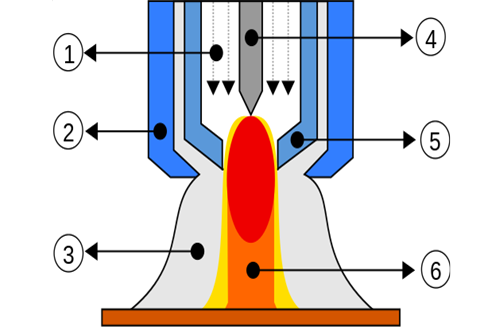
\includegraphics[width=\textwidth]{gorseller/ptaTorc}
\caption{PTA Torç}\label{fig:PtaTorc1}
\end{figure}
\lipsum[1-2]
\begin{table}
\centering
\caption{Deneme Tablosu.}\label{tab:den1}
\begin{tabular}{|l|l|l|}
\hline
sıra   & sayı   & toplam \\ \hline
1      & 2      & 3      \\ \hline
Kelime & deneme & son    \\ \hline
\end{tabular}
\end{table}


\section{Literatür Araştırması Birinci Derece Başlık}
\lipsum[1-2]
\begin{figure}[h]
\centering
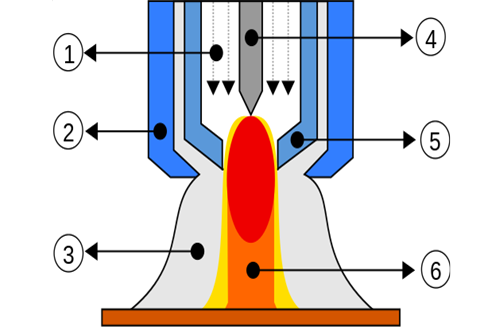
\includegraphics[width=\textwidth]{gorseller/ptaTorc}
\caption{PTA Torç}\label{fig:PtaTorc1}
\end{figure}
\lipsum[1-2]
\begin{table}
\centering
\caption{Deneme Tablosu.}\label{tab:den1}
\begin{tabular}{|l|l|l|}
\hline
sıra   & sayı   & toplam \\ \hline
1      & 2      & 3      \\ \hline
Kelime & deneme & son    \\ \hline
\end{tabular}
\end{table}
Teorem yazmak isterseniz:
\begin{theorem}[Öklid]
 İki noktadan bir ve yalnız bir doğru geçer.
\end{theorem}

İspat yazmak isterseniz:
\begin{ispat}[Tezin en önemli ispatı]
x=10
\end{ispat}

\subsection{Literatür Araştırması ikinci derece başlık}
\lipsum[1-2]
\begin{figure}[h]
\centering
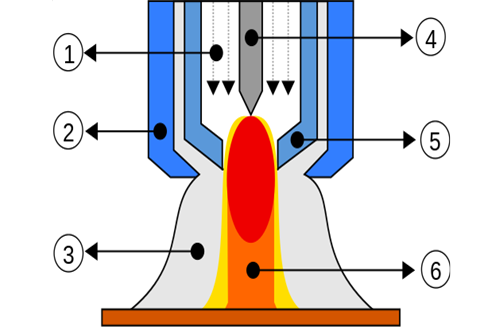
\includegraphics[width=\textwidth]{gorseller/ptaTorc}
\caption{PTA Torç}\label{fig:PtaTorc1}
\end{figure}
\lipsum[1-2]
\begin{table}
\centering
\caption{Deneme Tablosu.}\label{tab:den1}
\begin{tabular}{|l|l|l|}
\hline
sıra   & sayı   & toplam \\ \hline
1      & 2      & 3      \\ \hline
Kelime & deneme & son    \\ \hline
\end{tabular}
\end{table}

Teorem yazmak isterseniz:
\begin{theorem}[Öklid]
 İki noktadan bir ve yalnız bir doğru geçer.
\end{theorem}

İspat yazmak isterseniz:
\begin{ispat}[Tezin en önemli ispatı]
x=10
\end{ispat}

\subsubsection{Literatür araştırması dördüncü derece başlık}
\lipsum[1-2]
\begin{figure}[h]
\centering
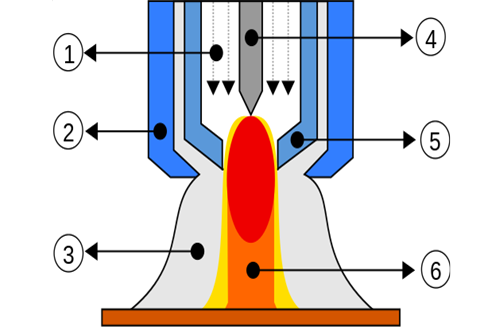
\includegraphics[width=\textwidth]{gorseller/ptaTorc}
\caption{PTA Torç}\label{fig:PtaTorc1}
\end{figure}
\lipsum[1-2]
\begin{table}
\centering
\caption{Deneme Tablosu.}\label{tab:den1}
\begin{tabular}{|l|l|l|}
\hline
sıra   & sayı   & toplam \\ \hline
1      & 2      & 3      \\ \hline
Kelime & deneme & son    \\ \hline
\end{tabular}
\end{table}

Teorem yazmak isterseniz:
\begin{theorem}[Öklid]
 İki noktadan bir ve yalnız bir doğru geçer.
\end{theorem}

İspat yazmak isterseniz:
\begin{ispat}[Tezin en önemli ispatı]
x=10
\end{ispat}